\documentclass[12pt]{article}

\usepackage{fullpage}
\usepackage{datetime}
\usepackage{amsfonts}
\usepackage{amsmath}

\usepackage{graphicx}
\usepackage{subcaption}

\usepackage{biblatex}
\addbibresource{./references.bib}

\usepackage{hyperref}

\title{Learning Neural Orientation Field for Volumetric Hair Reconstruction}
\author{
    Fangjun Zhou \\ fzhou48
    \and Zhenyu Zhang \\ zhenyuz5
    \and Weiran Xu \\ weiran
}
\date{\today}

\begin{document}
\maketitle


\section{Introduction}
% Project motivation

Reconstructing human hair is one of the most challenging yet critical process in rendering photorealistic digital human. Unlike other parts of the human body, human hair is highly detailed and often intertwined together. Therefore, it's difficult to use traditional photogrammetry method to reconstruct its structure.

Before machine learning model is used in this field, artists often hand crafted splines on skulls to represent hair strands. Each strand is then textured and rendered to mimic the hair volume. This workflow requires a lot of experience as it's non-trivial for artists to infer the final render result from hair stand splines. To reduce the workload and improve the accuracy of hair reconstruction, machine learning models are trained to generate hair strand from captured images.

In this work, we propose a new method capturing the hair structure by a 3D orientation field from $\mathbb{R}^{3} \rightarrow \mathbb{R}^{2}$ representing the hair growing direction and occupancy. On top of that, another occupancy field from $\mathbb{R}^{3} \rightarrow \mathbb{R}^{2}$ is learned to indicate hair and body occupancy. These mappings can be used later to generate hair stand directly by numerically integrating the orientation field. It can also be used as a latent variable to guide other generative models as mentioned in \cite{metzer_latent-nerf_2022}. We can fit this orientation field by a simple MLP. We then project the orientation field onto multiple camera view with a volumetric renderer. Since the screen space projection and volumetric rendering algorithms are differentiable, we are able to learn the orientation field from images from multiple camera angles.

%% TODO: Include the input and output of the model.
Our model is capable of predicting the output for unseen views using the hair orientation field observed from a limited number of camera viewpoints. During training, the model learns an implicit representation of the orientation field at each point in 3D space based on the existing 2D hair orientation fields. In the prediction phase, the implicit representation is leveraged to reconstruct, integrate, and project the orientation field for a target viewpoint. This process enables the prediction of the 2D hair orientation field for the unseen view, yielding the desired output.


\section{Related Work}

Previous attempts to achieve this goal mainly focused on learning-based hair strand generation. This includes some studies about single view hair synthesis \cite{saito_3d_2018, zheng_hairstep_2023, wu_neuralhdhair_2022, ma_single-view_nodate}. Since the image only contains hair structure from one viewing angle, it's impossible to reconstruct entire hair accurately. These models often use pretrained image encoders such as ResNet-50 \cite{saito_3d_2018} to encode the abstract hair style into a feature vector, then use generative models such as U-Net \cite{zheng_hairstep_2023}, VAE \cite{saito_3d_2018}, and diffusion models \cite{sklyarova_neural_2023} to generate the final strand. These models also struggle with generating curly hair as there's only limited information about growing direction after feature extraction.

In \cite{sklyarova_neural_2023} and \cite{rosu_neural_2022}, the authors also tried hair syntheses from multi-view images. However, these two studies still failed to capture finer detail.

Another study about this topic tried to tackle this problem by expanding the traditional PatchMatch MVS (PMVS) algorithm to a Line-based PatchMatch MVS (LPMVS) \cite{nam_strand-accurate_nodate}. This method, despite its high accuracy, doesn't capture the volumetric property of human hair.

Our work is highly inspired by NeRF \cite{mildenhall_nerf_2020}, a model used for 3D reconstruction from 2D images. However, our model differs in two major way.

In NeRF, the model fits a radiance field from $\mathbb{R}^{5} \rightarrow \mathbb{R}^{4}$. The input of the radiance function includes the sample position and view direction. However, since the orientation field our model fits is view-independent, the input space is only $\mathbb{R}^{3}$. This makes it easier for the model to capture more information from a smaller dataset.

On top of that, the volumetric renderer on orientation field also differs from the one on radiance field. When sampling the radiance field, NeRF only integrates the sampled color for each ray, while our model needs to project the sample orientation onto the filming plane and then integrate the projected orientation.


\section{Dataset}

%% TODO: Data generation. (Fangjun)

The dataset used by this project is generated by We choose a scene from Blender's Geometry Nodes-based hair system demo files (cite) and rendered a dataset of portraits. Each portrait comes with its camera information (including the intrinsic matrix and the transformation matrix). We write custom shaders to generate body masks and hair masks. Since we have the model information for each hair strand, we also generate the orientation of the hair in the camera space, represented by channels rgb; see Figure \ref{fig:dataset}. Our training set consists of 128 portraits and our test set consists of 16 portraits, all generated using the same scene as the training set, but with different camera positions.
\begin{figure}[h]
	\centering
	\begin{subfigure}{0.24\textwidth}
		\centering
		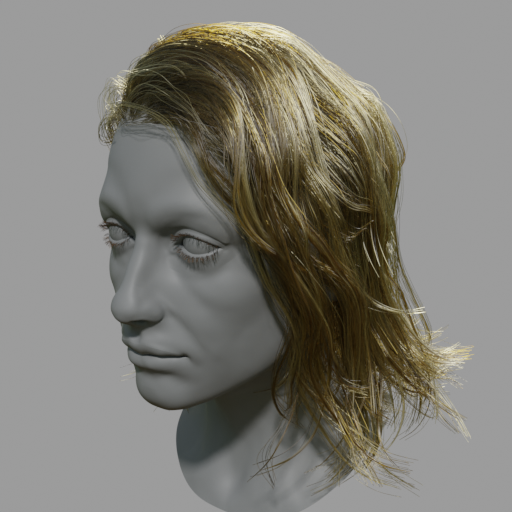
\includegraphics[width=\textwidth]{./images/0009_rendered.png}
		\caption{rendered}
	\end{subfigure}
	\hfill
	\begin{subfigure}{0.24\textwidth}
		\centering
		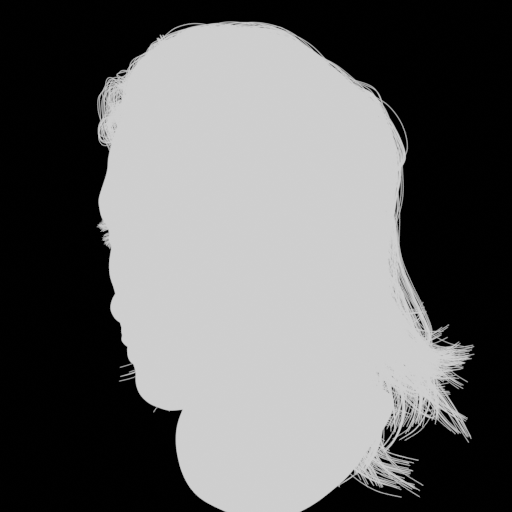
\includegraphics[width=\textwidth]{./images/0009_bodymask.png}
		\caption{body mask}
	\end{subfigure}
	\hfill
	\begin{subfigure}{0.24\textwidth}
		\centering
		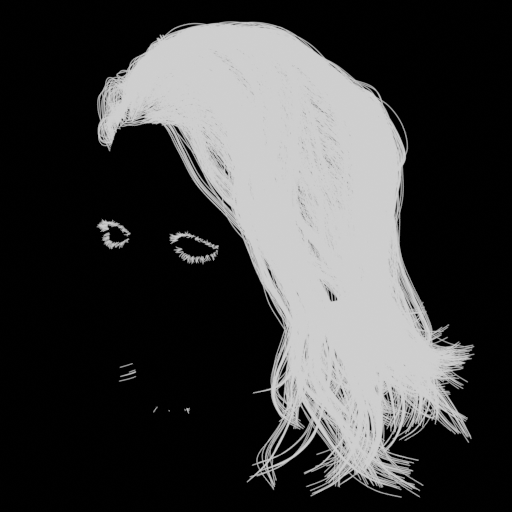
\includegraphics[width=\textwidth]{./images/0009_hairmask.png}
		\caption{hair mask}
	\end{subfigure}
	\hfill
	\begin{subfigure}{0.24\textwidth}
        \centering
        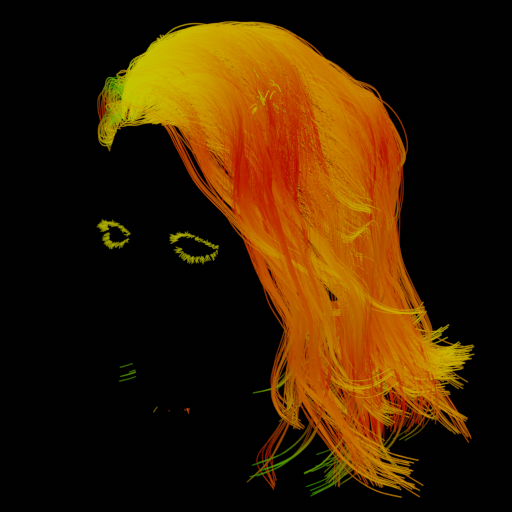
\includegraphics[width=\textwidth]{./images/0009_hairdir.png}
        \caption{hair orientation}
	\end{subfigure}

	\caption{dataset}
	\label{fig:dataset}
\end{figure}

\section{Method}

% TODO: Model structure. (Fangjun)
% TODO: Volumetric renderer for vector field. (Fangjun)
% TODO: Occupancy integration and mask loss. (Fangjun)
% TODO: Hierachical volumetric sampling for vector field. (Fangjun)

\subsection{Neural Orientation Field Model}

The neural orientation field model we proposed consists of multiple MLP layers and residual connections. The input of the network is the spatial coordinates $(x, y, z)$ of the point to be sampled. The output is the normalized orientation of the hair $(\theta, \phi)$, as well as the opacity parameter $\sigma = (\sigma_{void}, \sigma_{hair}, \sigma_{body})$. A softmax layer is used to make $\Vert \sigma \Vert_{2} = 1$.

\subsection{Volumetric Rendering of a Neural Orientation Field}

For each camera in the scene, we can emit camera rays for each pixel on the filming plane. Then, hair orientation and occupancy can be sampled along the camera ray. Given the camera view matrix $V \in \mathbb{R}_{4x4}$, the normalized orientation vector in homogeneous coordinate $\mathbf{o} \in \mathbb{R}^{4}$ can be projected to the view space by $\mathbf{o}_{view} = V\mathbf{o}$.

To project the orientation vectors onto screen space, we need to apply camera projection to the view space vectors. However, as we choose pinhole camera as our camera model, the projected vectors are independent of the camera parameters. In this cases, the screen space projection of the view space orientation is $\mathbf{o}_{screen}$

\begin{align}
	P &= \begin{bmatrix}
        1 & 0 & 0 & 0 \\
        0 & 1 & 0 & 0 \\
        0 & 0 & 0 & 0 \\
        0 & 0 & 0 & 0
    \end{bmatrix} \\
	\mathbf{o}_{screen} & = P\mathbf{o}_{view}
\end{align}

Similar to the volumetric rendering function defined in NeRF \cite{mildenhall_nerf_2020}, our rendering function for screen space orientation can be written as

\begin{align}
	O(\mathbf{r}) & = \int_{t_{n}}^{t_{f}} T(t) \sigma_{hair}(\mathbf{r}(t)) P V \mathbf{o}(\mathbf{r}(t), \mathbf{d}) dt \\
	T(t) & = exp(-\int_{t_{n}}^{t_{f}} \sigma_{hair}(\mathbf{r}(s)) ds)
\end{align}

One important difference between our model and NeRF is we use two separate occupancy for body and hair, while in NeRF one occupancy is used to integrate camera rays. In our case, camera rays can be blocked by face and body that doesn't contribute to the final hair orientation field. These parts are marked red in the preprocessing step s demonstrated in Figure \ref{fig:image_prep}. When training the model, we integrate the 2D hair orientation using the aforementioned volumetric render function. We also run a traditional NeRF volumetric renderer to integrate the body occupancy to generate the body mask. The final loss is defined as the combination of two losses.

\section{Experiment}

\subsection{Setup}
% TODO: Baseline & Model setup

\subsubsection{Datasets} 

To perform more precise model evaluation, we generated a dataset using Blender. For the same individual, the dataset includes 144 RGB hair photos with a resolution of 512x512 taken from different viewpoints, corresponding body and hair masks, camera parameters and pose matrices, as well as 2D hair orientations observed from the camera positions. The dataset for each individual is split into a training set with 128 images, a validation set with 16 images, and a test set with 16 images. 

\subsubsection{Metrics} 
We use PSNR (Peak Signal-to-Noise Ratio) for evaluation. The model performs reconstruction on unseen viewpoints to obtain the reconstructed 2D hair orientation for these viewpoints. The vector field is compared with the Ground Truth 2D hair orientation by calculating the MSE, and the MSEs from all different viewpoints are averaged. This average MSE is then used to compute the overall PSNR metric. The complete formula is as follows:

\begin{align*}
    \text{MSE}_k &= \frac{1}{M \cdot N \cdot 2} \sum_{i=1}^M \sum_{j=1}^N \sum_{c=1}^2 \left(I_k (i,j,c) - K_k(i,j,c) \right)^2 \\
    \text{MSE}_\text{avg} &= \frac{1}{N_\text{images}} \sum_{k=1}^{N_\text{images}}\text{MSE}_k \\
    \text{PSNR}_\text{avg} &= 10 \cdot \log_{10} \left( \frac{\text{MAX}^2}{\text{MSE}_{\text{avg}}} \right)
\end{align*}

where $\text{MSE}_k$ is the MSE of image $k$ and its ground truth, $I_k$ and $K_k$ are the reconstructed 2D hair orientation for image $k$, $N$ and $M$ is the height and weight of the image, $N_\text{images}$ is the number of images, $\text{MSE}_\text{avg}$ is the average MSE of these image, MAX is the maximum possible value of each pixel (here we use 8-bit image, so it is 255), and $\text{PSNR}_\text{avg}$ is our final PSNR value.

\subsubsection{Baseline Method}
We trained a NeRF model to represent the hair structure as a radiance field, leveraging it to infer hair orientation. Since NeRF does not inherently encode orientation information, we relied on HairStep to predict orientation. Observed that the output of NeRF is often blurred, consistent with findings from the original NeRF paper \cite{mildenhall_nerf_2020}, which noted that NeRF tends to capture low-frequency features early in training, making HairStep difficult to segment out hair and output reasonable hair direction, thus unable to maintain relevant direction information; see Figure \ref{fig:nerf_hairstep}.
\begin{figure}[h]
    \centering
    \begin{subfigure}{0.48\textwidth}
        \centering
        \begin{subfigure}{0.48\textwidth}
            \centering
            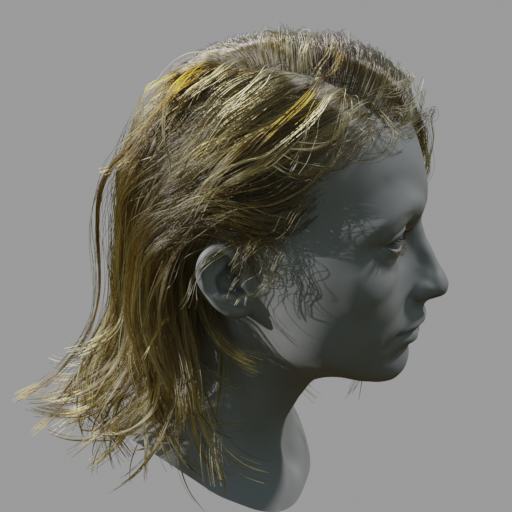
\includegraphics[width=\textwidth]{./images/test_6_rendered.png}
        \end{subfigure}
        \hfill
        \begin{subfigure}{0.48\textwidth}
            \centering
            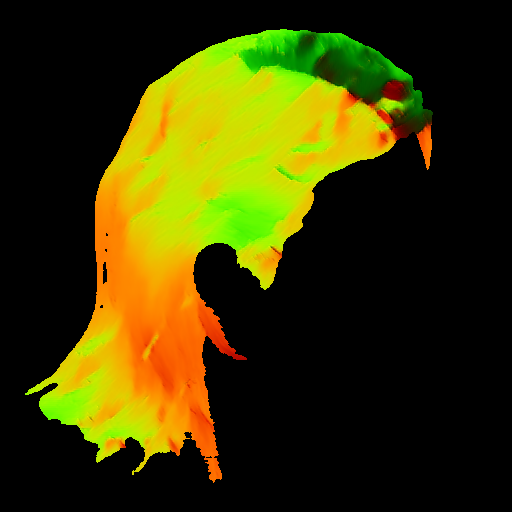
\includegraphics[width=\textwidth]{./images/test_6_hairstep.jpg}
        \end{subfigure}
        \caption{ground truth with hairstep}
    \end{subfigure}
    \hfill
    \begin{subfigure}{0.48\textwidth}
        \begin{subfigure}{0.48\textwidth}
            \centering
            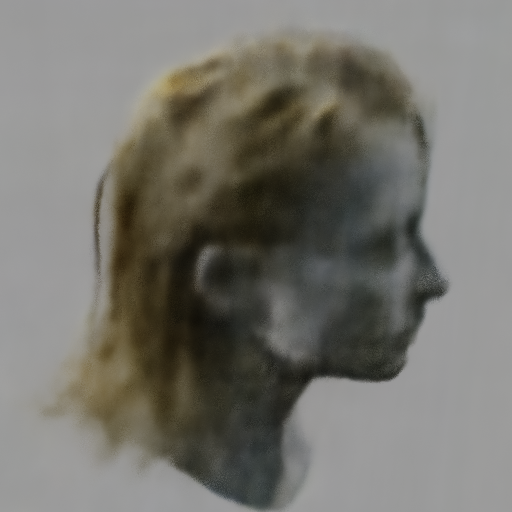
\includegraphics[width=\textwidth]{./images/pred_6_nerf.png}
        \end{subfigure}
        \hfill
        \begin{subfigure}{0.48\textwidth}
            \centering
            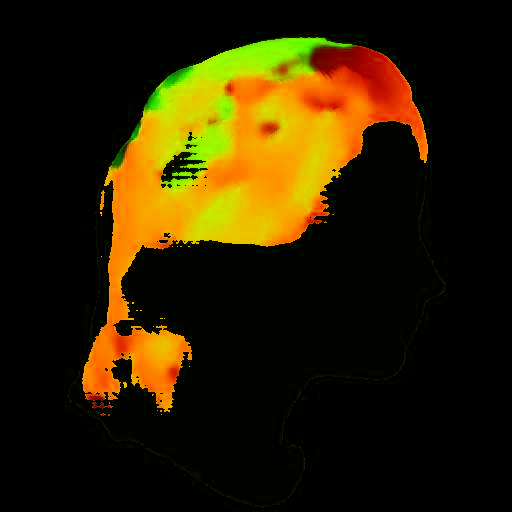
\includegraphics[width=\textwidth]{./images/pred_6_hairstep.jpg}
        \end{subfigure}
        \caption{nerf pred with hairstep}
    \end{subfigure}

    \caption{NeRF's output on evaluation set, blurry output makes }
    \label{fig:nerf_hairstep}
\end{figure}

\subsubsection{Implementation Details}


\subsection{Observation}


% TODO: Experiement setup. (Fangjun, Zhenyu)
% TODO: Experiement observations. (Fangjun)
% TODO: Baseline setup.

% \subsection{Metrics}

% The Peak Signal-to-Noise Ratio (PSNR) is a widely used metric in signal processing to assess image similarity, particularly in image reconstruction tasks. It effectively represents the Mean Squared Error (MSE) between two images in a 2D context.

We also observed signs of overfitting in NeRF, with the PSNR on the evaluation set stabilizing around 1000 batches. We aim to address this with regularization methods (WIP). Additionally, we hypothesize that the model may converge faster on a smaller dataset, given that the hair orientation field we aim to fit is view-independent and should not vary with camera position. As the outcome is evident, we opted not to measure PSNR for the NeRF baseline.

\section{Result}

% TODO: Result. (Weiran, Zhenyu)

\printbibliography

\newpage

\section{Contribution}

\subsection{Fangjun Zhou}

Wrote preprocessing script that uses COLMAP to extract features and camera poses. Wrote colmap\_visualizer using imagui and pyvista to help visualize the extracted point cloud / camera position. Wrote helper methods to construct camera rays for NeRF training. Rendered hoover tower dataset in Blender. Implement and trained NeRF baseline. Derive orientation vector projection volumetric render function. Wrote method section in the milestone report.

\subsection{Weiran Xu}

Contributed to building the human portrait dataset and applied HairStep for image preprocessing and hair strand direction extraction, preparing the data for analysis. Also wrote part of experiment section in the milestone report, detailing methodology and preliminary findings.

\subsection{Zhenyu Zhang}

Responsible for refactoring Tiny NeRF, do the training and testing related to Tiny NeRF, and implementing the code for 3D vector field reconstruction of hair growth. This included model code, loss computation code, camera view transformation and coordinate system conversion code, as well as the code of calculations for remapping 3D vectors in space to the camera frame.

\end{document}
